\begin{frame}
	\myheading{Module 9.2 : Unsupervised pre-training}
\end{frame}

%%%%%%%%%%%%%%%%%%%%%%%%%%%%%%%%%%%%%%%%%%%%%%%%%%%%%%%%%%%%%%%%%%%%%%%%%%%%%%%%%%%%%%%%%

\begin{frame}
	
	\begin{block}{}
		\begin{itemize}
			\justifying
			\item<1-> What has changed now? How did Deep Learning become so popular despite this problem with training large networks?
			\item<2-> Well, until 2006 it wasn't so popular
			\item<3-> The field got revived after the seminal work of Hinton and Salakhutdinov in 2006
		\end{itemize}
	\end{block}
	
	\footnotetext[1]{G. E. Hinton and R. R. Salakhutdinov. Reducing the dimensionality of data with neural networks. Science, 313(5786):504–507, July 2006.}
\end{frame}

%%%%%%%%%%%%%%%%%%%%%%%%%%%%%%%%%%%%%%%%%%%%%%%%%%%%%%%%%%%%%%%%%%%%%%%%%%%%%%%%%%%%%%%%%

\begin{frame}
	Let's look at the idea of unsupervised pre-training introduced in this paper ... \onslide<2->{(note that in this paper they introduced the idea in the context of RBMs but we will discuss it in the context of Autoencoders)}
\end{frame}

%%%%%%%%%%%%%%%%%%%%%%%%%%%%%%%%%%%%%%%%%%%%%%%%%%%%%%%%%%%%%%%%%%%%%%%%%%%%%%%%%%%%%%%%%

\begin{frame}
	\begin{columns}
		
		\column{0.3\textwidth}
		%\begin{overlayarea}{\textwidth}{\textheight}
		\vspace{1cm}
				
		\only<1->{
			\begin{center}
				\tikzstyle{input_neuron}=[circle,draw=red!50,fill=red!10,thick,minimum size=6mm]
\tikzstyle{hidden_neuron}=[circle,draw=blue!50,fill=cyan!10,thick,minimum size=6mm]
\tikzstyle{output_neuron}=[circle,draw=green!50,fill=green!10,thick,minimum size=6mm]

\tikzstyle{input}=[circle,draw=black!50,fill=black!20,thick,minimum size=6mm]
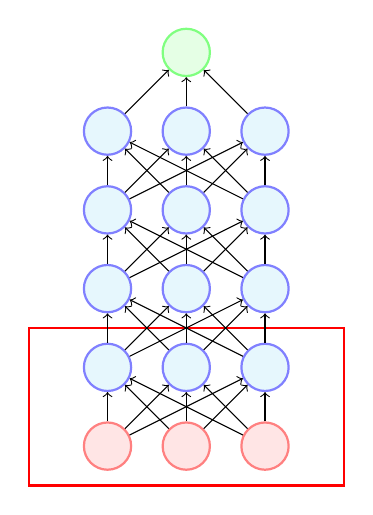
\begin{tikzpicture}
					
	\node [input_neuron] (neuron01) at (7,4.5){} ;
	\node [input_neuron] (neuron02) at (8,4.5){};
	\node [input_neuron] (neuron03) at (9,4.5){} ;
	\node [hidden_neuron] (neuron51) at (7,5.5){}  ;
	\node [hidden_neuron] (neuron52) at (8,5.5){}  ;
	\node [hidden_neuron] (neuron53) at (9,5.5){}  ;
	
	\node [hidden_neuron] (neuron11) at (7,6.5){}  ;
	\node [hidden_neuron] (neuron12) at (8,6.5){}  ;
	\node [hidden_neuron] (neuron13) at (9,6.5){}  ;
	\node [hidden_neuron] (neuron21) at (7,7.5){}  ;
	\node [hidden_neuron] (neuron22) at (8,7.5){}  ;
	\node [hidden_neuron] (neuron23) at (9,7.5){}  ;
	\node [hidden_neuron] (neuron31) at (7,8.5){}  ;
	\node [hidden_neuron] (neuron32) at (8,8.5){}  ;
	\node [hidden_neuron] (neuron33) at (9,8.5){}  ;
	\node [output_neuron] (neuron4) at (8,9.5){}  ;
	
	\draw[red!100,thick,solid] (6,4) rectangle (10,6);
	\draw[->](neuron01) -- (neuron51);
	\draw[->](neuron01) -- (neuron52);
	\draw[->](neuron01) -- (neuron53);
	\draw[->](neuron02) -- (neuron51);
	\draw[->](neuron02) -- (neuron52);
	\draw[->](neuron02) -- (neuron53);
	\draw[->](neuron03) -- (neuron51);
	\draw[->](neuron03) -- (neuron52);
	\draw[->](neuron03) -- (neuron53);
	
	\draw[->](neuron51) -- (neuron11);
	\draw[->](neuron51) -- (neuron12);
	\draw[->](neuron51) -- (neuron13);
	\draw[->](neuron52) -- (neuron11);
	\draw[->](neuron52) -- (neuron12);
	\draw[->](neuron52) -- (neuron13);
	\draw[->](neuron53) -- (neuron11);
	\draw[->](neuron53) -- (neuron12);
	\draw[->](neuron53) -- (neuron13);
	
	\draw [->] (neuron11) -- (neuron21);
	\draw [->] (neuron11) -- (neuron22);
	\draw [->] (neuron11) -- (neuron23);
	\draw [->] (neuron12) -- (neuron21);
	\draw [->] (neuron12) -- (neuron22);
	\draw [->] (neuron12) -- (neuron23);
	\draw [->] (neuron13) -- (neuron21);
	\draw [->] (neuron13) -- (neuron22);
	\draw [->] (neuron13) -- (neuron23);
	
	\draw [->] (neuron21) -- (neuron31);
	\draw [->] (neuron21) -- (neuron32);
	\draw [->] (neuron21) -- (neuron33);
	\draw [->] (neuron22) -- (neuron31);
	\draw [->] (neuron22) -- (neuron32);
	\draw [->] (neuron22) -- (neuron33);
	\draw [->] (neuron23) -- (neuron31);
	\draw [->] (neuron23) -- (neuron32);
	\draw [->] (neuron23) -- (neuron33);
	
	\draw [->] (neuron31) -- (neuron4);
	\draw [->] (neuron32) -- (neuron4);
	\draw [->] (neuron33) -- (neuron4);
	
\end{tikzpicture}
			\end{center}
		}
						
		\column{0.3\textwidth}

		
		\only<4-7>{
			\begin{center}
				\tikzstyle{input_neuron}=[circle,draw=red!50,fill=red!10,thick,minimum size=6mm]
\tikzstyle{hidden_neuron}=[circle,draw=blue!50,fill=cyan!10,thick,minimum size=6mm]
\tikzstyle{output_neuron}=[circle,draw=green!50,fill=green!10,thick,minimum size=6mm]
\tikzstyle{input}=[circle,draw=black!50,fill=black!20,thick,minimum size=6mm]

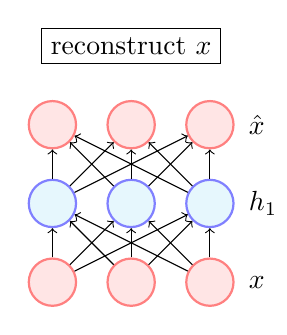
\begin{tikzpicture}
		
	\node [input_neuron] (neuron11) at (7,5) {}  ;
	\node [input_neuron] (neuron12) at (8,5) {}  ;
	\node [input_neuron] (neuron13) at (9,5) {}  ;
	\node [hidden_neuron] (neuron21) at (7,6) {}  ;
	\node [hidden_neuron] (neuron22) at (8,6) {}  ;
	\node [hidden_neuron] (neuron23) at (9,6) {}  ;
	\node [input_neuron] (neuron31) at (7,7) {}  ;
	\node [input_neuron] (neuron32) at (8,7) {}  ;
	\node [input_neuron] (neuron33) at (9,7) {}  ;
	
	\node[text width=0.01cm] at (9.5,7) {$\hat{x}$};
	\node[text width=0.01cm] at (9.5,6) {$h_{1}$};
	\node[text width=0.01cm] at (9.5,5) {$x$};
	
	\node[draw,align = center] at (8,8) {reconstruct $x$};
	
	\draw [->] (neuron11) -- (neuron21);
	\draw [->] (neuron11) -- (neuron22);
	\draw [->] (neuron11) -- (neuron23);
	\draw [->] (neuron12) -- (neuron21);
	\draw [->] (neuron12) -- (neuron22);
	\draw [->] (neuron12) -- (neuron23);
	\draw [->] (neuron13) -- (neuron21);
	\draw [->] (neuron13) -- (neuron22);
	\draw [->] (neuron13) -- (neuron23);
	
	\draw [->] (neuron21) -- (neuron31);
	\draw [->] (neuron21) -- (neuron32);
	\draw [->] (neuron21) -- (neuron33);
	\draw [->] (neuron22) -- (neuron31);
	\draw [->] (neuron22) -- (neuron32);
	\draw [->] (neuron22) -- (neuron33);
	\draw [->] (neuron23) -- (neuron31);
	\draw [->] (neuron23) -- (neuron32);
	\draw [->] (neuron23) -- (neuron33);
	
\end{tikzpicture}
				\begin{align*}
					\min {\hspace{.3mm}} \frac{1}{m}\sum_{i=1}^{m}\sum_{j=1}^{n} (\hat{x}_{ij} - x_{ij})^{2} 
				\end{align*}
			\end{center}
			
		}
		
		
		\only<8->{
			
			\begin{center}
				\tikzstyle{input_neuron}=[circle,draw=red!50,fill=red!10,thick,minimum size=6mm]
\tikzstyle{hidden_neuron}=[circle,draw=blue!50,fill=cyan!10,thick,minimum size=6mm]
\tikzstyle{output_neuron}=[circle,draw=green!50,fill=green!10,thick,minimum size=6mm]
\tikzstyle{input}=[circle,draw=black!50,fill=black!20,thick,minimum size=6mm]
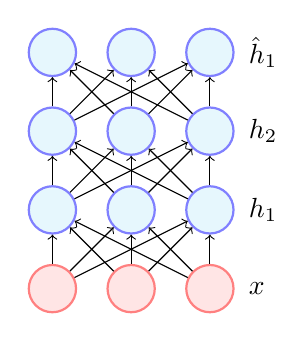
\begin{tikzpicture}	
	
	\node [input_neuron] (neuron11) at (7,2.5){}  ;
	\node [input_neuron] (neuron12) at (8,2.5){}  ;
	\node [input_neuron] (neuron13) at (9,2.5){}  ;
	\node [hidden_neuron] (neuron21) at (7,3.5){}  ;
	\node [hidden_neuron] (neuron22) at (8,3.5){}  ;
	\node [hidden_neuron] (neuron23) at (9,3.5){}  ;
	\node [hidden_neuron] (neuron31) at (7,4.5){}  ;
	\node [hidden_neuron] (neuron32) at (8,4.5){}  ;
	\node [hidden_neuron] (neuron33) at (9,4.5){}  ;
	\node [hidden_neuron] (neuron41) at (7,5.5){}  ;
	\node [hidden_neuron] (neuron42) at (8,5.5){}  ;
	\node [hidden_neuron] (neuron43) at (9,5.5){}  ;
	
	%\draw[red!100,thick,solid] (6.5,2) rectangle (9.5,4);
	\node[text width=0.01cm] at (9.5,5.5) {$\hat{h}_1$};
	\node[text width=0.01cm] at (9.5,4.5) {$h_{2}$};
	\node[text width=0.01cm] at (9.5,3.5) {$h_{1}$};
	\node[text width=0.01cm] at (9.5,2.5) {$x$};
	
	\draw [->] (neuron11) -- (neuron21);
	\draw [->] (neuron11) -- (neuron22);
	\draw [->] (neuron11) -- (neuron23);
	\draw [->] (neuron12) -- (neuron21);
	\draw [->] (neuron12) -- (neuron22);
	\draw [->] (neuron12) -- (neuron23);
	\draw [->] (neuron13) -- (neuron21);
	\draw [->] (neuron13) -- (neuron22);
	\draw [->] (neuron13) -- (neuron23);
	
	\draw [->] (neuron21) -- (neuron31);
	\draw [->] (neuron21) -- (neuron32);
	\draw [->] (neuron21) -- (neuron33);
	\draw [->] (neuron22) -- (neuron31);
	\draw [->] (neuron22) -- (neuron32);
	\draw [->] (neuron22) -- (neuron33);
	\draw [->] (neuron23) -- (neuron31);
	\draw [->] (neuron23) -- (neuron32);
	\draw [->] (neuron23) -- (neuron33);
	
	\draw [->] (neuron31) -- (neuron41);
	\draw [->] (neuron31) -- (neuron42);
	\draw [->] (neuron31) -- (neuron43);
	\draw [->] (neuron32) -- (neuron41);
	\draw [->] (neuron32) -- (neuron42);
	\draw [->] (neuron32) -- (neuron43);
	\draw [->] (neuron33) -- (neuron41);
	\draw [->] (neuron33) -- (neuron42);
	\draw [->] (neuron33) -- (neuron43);
	
\end{tikzpicture}
				\begin{align*}
					\min {\hspace{.3mm}} \frac{1}{m}\sum_{i=1}^{m}\sum_{j=1}^{n} (\hat{h}_{{1}_{ij}} - h_{{1}_{ij}})^{2}
				\end{align*}
				
			\end{center}
		}
		
		
		%\end{overlayarea}
		
		\column{0.5\textwidth}
		\only<1-6>{
			\begin{itemize}[<+(0)->]
				\justifying 
				\item Consider the deep neural network shown in this figure
				\item Let us focus on the first two layers of the network ($x$ and $h_1$) 
				\item We will first train the weights between these two layers using an \textbf{unsupervised objective}
				\item Note that we are trying to reconstruct the input ($x$) from the hidden representation ($h_1$)
				\item We refer to this as an unsupervised objective because it does not involve the output label ($y$) and only uses the input data ($x$)
				      %\item Now,fix the weights for the first layer and repeat the autoencoder training for the second layer
				      %\item Continue till the last hidden layer (i.e. the layer before the output layer)
			\end{itemize}
		}
		
		
		\only<7->{
			\begin{itemize}[<+(6)->]
				\justifying     
				\item At the end of this step, the weights in layer 1 are trained such that $h_1$ captures an abstract representation of the input $x$ 
				\item We now fix the weights in layer 1 and repeat the same process with layer 2
				\item At the end of this step, the weights in layer 2 are trained such that $h_2$ captures an abstract representation of $h_1$
				\item We continue this process till the last hidden layer (\textit{i.e.,} the layer before the output layer) so that each successive layer captures an abstract representation of the previous layer
				      %\item Now,fix the weights for the first layer and repeat the autoencoder training for the second layer
				      %\item Continue till the last hidden layer (i.e. the layer before the output layer)
			\end{itemize}
		}
		
	\end{columns}
\end{frame}

%%%%%%%%%%%%%%%%%%%%%%%%%%%%%%%%%%%%%%%%%%%%%%%%%%%%%%%%%%%%%%%%%%%%%%%%%%%%%%%%%%%%%%%%%

\begin{frame}
	\begin{columns}
		
		\column{0.5\textwidth}
		\begin{overlayarea}{\textwidth}{\textheight}
						
			\begin{center}
				\tikzstyle{input_neuron}=[circle,draw=red!50,fill=orange!10,thick,minimum size=6mm]
\tikzstyle{hidden_neuron}=[circle,draw=blue!50,fill=blue!10,thick,minimum size=1mm]
\tikzstyle{output_neuron}=[circle,draw=green!50,fill=green!20,thick,minimum size=1mm]
\tikzstyle{input}=[circle,draw=black!50,fill=black!20,thick,minimum size=1mm]

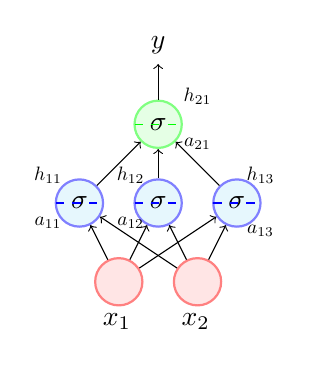
\begin{tikzpicture}
	
	\node [input_neuron] (in1) at (6.5,1)  {} ;
	\node [input_neuron] (in2) at (7.5,1)  {} ;
	%\node (input1) at (6.5,0)  {$x_{1}$};
	%\node (input2) at (7.5,0)  {$x_{2}$};
	\node (output1) at (7,4)  {$y$};
	\node [hidden_neuron] (h1) at (6,2)  {$\sigma$};
	\node [hidden_neuron] (h2) at (7,2)  {$\sigma$};
	\node [hidden_neuron] (h3) at (8,2)  {$\sigma$};
	\node [output_neuron] (o1) at (7,3)  {$\sigma$};
	
	\node[text width=0.005cm] at (6.3,0.5) {$x_{1}$};
	\node[text width=0.005cm] at (7.3,0.5) {$x_{2}$};
	
	%\draw [->] (input1) -- (in1);
	%\draw [->] (input2) -- (in2);
	
	\draw [->] (in1) -- (h1);
	\draw [->] (in1) -- (h2);
	\draw [->] (in1) -- (h3);
	\draw [->] (in2) -- (h1);
	\draw [->] (in2) -- (h2);
	\draw [->] (in2) -- (h3);
	
	\draw [->] (h1) -- (o1);
	\draw [->] (h2) -- (o1);
	\draw [->] (h3) -- (o1);
	
	\draw [->] (o1) -- (output1);
	
	\draw[green,dashed] (6.7,3) -- (7.3,3);
	\draw[blue,dashed] (5.7,2) -- (6.3,2);
	\draw[blue,dashed] (6.7,2) -- (7.3,2);
	\draw[blue,dashed] (7.7,2) -- (8.3,2);
	
	\node (formula)[scale=.7] at (7.5,3.35) {$h_{21}$};
	\node (formula)[scale=.7] at (7.5,2.75) {$a_{21}$};
	
	\node (formula)[scale=.7] at (5.6,2.35) {$h_{11}$};
	\node (formula)[scale=.7] at (6.65,2.35) {$h_{12}$};
	\node (formula)[scale=.7] at (8.3,2.35) {$h_{13}$};
	
	\node (formula)[scale=.7] at (5.6,1.75) {$a_{11}$};
	\node (formula)[scale=.7] at (6.65,1.75) {$a_{12}$};
	\node (formula)[scale=.7] at (8.3,1.65) {$a_{13}$};
	
\end{tikzpicture}
			\end{center}
			\vspace{-1em}
			\begin{align*}
				\min_{\theta} \hspace{.3mm}\frac{1}{m} \sum_{i=1}^{m} (y_{i} - f(x_i))^{2} 
			\end{align*}
			
			
		\end{overlayarea}
		\column{0.5\textwidth}
		
		\begin{itemize}[<+(0)->]
			\justifying
			%\item At the end of this process the weights of all the layers have been initialised such that the network now has a better class-independent representation of the data (class independent because we have not used the class labels $y$ anywhere)
			\item After this layerwise pre-training, we add the output layer and train the whole network using the task specific objective
			\item Note that, in effect we have initialized the weights of the network using the greedy unsupervised objective and are now fine tuning these weights using the supervised objective 
		\end{itemize}
		
	\end{columns}
\end{frame}

%%%%%%%%%%%%%%%%%%%%%%%%%%%%%%%%%%%%%%%%%%%%%%%%%%%%%%%%%%%%%%%%%%%%%%%%%%%%%%%%%%%%%%%%%

\begin{frame}
	\begin{flushleft}
		Why does this work better?\pause
	\end{flushleft}
	\vspace{-1em}
	\begin{itemize}
		\justifying
		\item<2-> Is it because of better optimization?
		\item<3-> Is it because of better regularization?\pause
	\end{itemize}
	\onslide<4->{\begin{flushleft}
				Let's see what these two questions mean and try to answer them based on some (among many) existing studies$^{1,2}$
			\end{flushleft}	
	}
	
	\onslide<4->{\footnotetext[1]{The difficulty of training deep architectures and effect of unsupervised pre-training - Erhan et al,2009}}
	\onslide<4->{\footnotetext[2]{Exploring Strategies for Training Deep Neural Networks, Larocelle et al,2009}}
	
	
\end{frame}

%%%%%%%%%%%%%%%%%%%%%%%%%%%%%%%%%%%%%%%%%%%%%%%%%%%%%%%%%%%%%%%%%%%%%%%%%%%%%%%%%%%%%%%%%

\begin{frame}
\begin{flushleft}
	Why does this work better?
\end{flushleft}
	\vspace{-1em}
	\begin{itemize}
		\justifying
		\item \textcolor {red}{Is it because of better optimization?}
		\item Is it because of better regularization?
	\end{itemize}
	
\end{frame}

%%%%%%%%%%%%%%%%%%%%%%%%%%%%%%%%%%%%%%%%%%%%%%%%%%%%%%%%%%%%%%%%%%%%%%%%%%%%%%%%%%%%%%%%%

\begin{frame}
	\begin{itemize}
		\justifying
		\item What is the optimization problem that we are trying to solve?
		      \onslide<2->{
		      	\begin{align*}
		      		\text{minimize} \hspace{0.65em} \displaystyle\mathscr{L(\theta)}=\frac{1}{m}\sum_{i=1}^{m} (y_{i} - f(x_{i}))^{2} 
		      	\end{align*}
		      }
		      \item<3-> Is it the case that in the absence of unsupervised pre-training we are not able to drive $\displaystyle\mathscr{L (\theta)}$ to 0 even for the training data (hence poor optimization) ?
		      \item<4-> Let us see this in more detail ... 
	\end{itemize}
	
\end{frame}    

%%%%%%%%%%%%%%%%%%%%%%%%%%%%%%%%%%%%%%%%%%%%%%%%%%%%%%%%%%%%%%%%%%%%%%%%%%%%%%%%%%%%%%%%%

\begin{frame}
	\begin{columns}
		\begin{column} {0.5\textwidth}
			\begin{figure}
				\includegraphics[scale= 0.4]{images/surface_.jpeg}
			\end{figure}
			
		\end{column}
		\begin{column}{0.5\textwidth}
			\begin{itemize}[<+->]
				\justifying
				\item The error surface of the supervised objective of a Deep Neural Network is highly non-convex
				\item With many hills and plateaus and valleys 
				\item Given that large capacity of DNNs it is still easy to land in one of these 0 error regions
				\item Indeed Larochelle et.al.$^1$ show that if the last layer has large capacity then $\displaystyle\mathscr{L (\theta)}$ goes to 0 even without pre-training
				\item However, if the capacity of the network is small, unsupervised pre-training helps
			\end{itemize}    
			
		\end{column}
		
	\end{columns}
	\footnotetext[1]{Exploring Strategies for Training Deep Neural Networks, Larocelle et al,2009}
\end{frame}

\begin{frame}
\begin{flushleft}
	Why does this work better?
\end{flushleft}
	\vspace{-1em}
	\begin{itemize}
		\justifying
		\item Is it because of better optimization?
		\item \textcolor{red}{Is it because of better regularization?}
	\end{itemize}
	
\end{frame}

%%%%%%%%%%%%%%%%%%%%%%%%%%%%%%%%%%%%%%%%%%%%%%%%%%%%%%%%%%%%%%%%%%%%%%%%%%%%%%%%%%%%%%%%%

\begin{frame}
	\begin{columns}
		\begin{column} {0.5\textwidth}
			\begin{center}
				\onslide<3->{ \includegraphics[scale= 0.2]{images/l1_l2.png}
				}
				    
				
			\end{center}
			
		\end{column}
		\begin{column}{0.5\textwidth}
			\begin{itemize}
				\justifying
				\item<1-> What does regularization do? \onslide<2-> {It constrains the weights to certain regions of the parameter space}
				\item<3-> L-1 regularization: constrains most weights to be 0 
				\item<4-> L-2 regularization: prevents most weights from taking large values 
			\end{itemize}
			
		\end{column}
		
	\end{columns}
	\footnotetext[1]{Image Source:The Elements of Statistical Learning-T. Hastie, R. Tibshirani, and J. Friedman, Pg 71 }
\end{frame}

%%%%%%%%%%%%%%%%%%%%%%%%%%%%%%%%%%%%%%%%%%%%%%%%%%%%%%%%%%%%%%%%%%%%%%%%%%%%%%%%%%%%%%%%%

\begin{frame}
	\begin{columns}
		\begin{column} {0.5\textwidth}
			\begin{overlayarea}{\textwidth}{\textheight}
				
				\begin{itemize}
					\justifying
					\item<3-> \textbf{Unsupervised objective:}
					
					\only<3->{
						\begin{align*}
							\Omega(\theta) = \frac{1}{m}\sum_{i=1}^{m} \sum_{j=1}^{n}(x_{ij} - \hat{x}_{ij})^{2} 
						\end{align*}
					}
					
					\item<4-> We can think of this unsupervised objective as an additional constraint on the optimization problem
					\item<5-> \textbf{Supervised objective:}
					
					\only<5->{
						\begin{align*}
							\mathscr{L}(\theta) = \frac{1}{m}\sum_{i=1}^{m} (y_{i} - f(x_{i}))^{2} 
						\end{align*}
					}
					
				\end{itemize}
			\end{overlayarea}
		\end{column}
		\begin{column}{0.5\textwidth}
			\begin{overlayarea}{\textwidth}{\textheight}
				
				\begin{itemize}
					\justifying
					\item<1-> Indeed, pre-training constrains the weights to lie in only certain regions of the parameter space
					\item<2-> Specifically, it constrains the weights to lie in regions where the characteristics of the data are captured well (as governed by the unsupervised objective)
					\item<5-> This unsupervised objective ensures that that the learning is not greedy w.r.t. the supervised objective (and also satisfies the unsupervised objective)
				\end{itemize}
			\end{overlayarea}
		\end{column}
		
	\end{columns}
\end{frame}

%%%%%%%%%%%%%%%%%%%%%%%%%%%%%%%%%%%%%%%%%%%%%%%%%%%%%%%%%%%%%%%%%%%%%%%%%%%%%%%%%%%%%%%%%

\begin{frame}
	\begin{columns}
		\begin{column} {0.5\textwidth}
			\begin{center}
				\onslide<2->{ \includegraphics[scale= 0.23]{images/erhan09_slide8.png} }
				
			\end{center}
		\end{column}
		
		\begin{column}{0.5\textwidth}
			
			\begin{itemize}[<+->]
				\justifying
				\item Some other experiments have also shown that pre-training is more robust to random initializations
				\item One accepted hypothesis is that pre-training leads to better weight initializations (so that the layers capture the internal characteristics of the data)
			\end{itemize}
			
		\end{column}
		
	\end{columns}
	\footnotetext[1]{The difficulty of training deep architectures and effect of unsupervised pre-training - Erhan et al,2009}
		
\end{frame}

%%%%%%%%%%%%%%%%%%%%%%%%%%%%%%%%%%%%%%%%%%%%%%%%%%%%%%%%%%%%%%%%%%%%%%%%%%%%%%%%%%%%%%%%%
\if 0
\begin{frame}
	\begin{columns}
				
		\column{0.5\textwidth}
		\begin{itemize}[<+(1)->]
			\justifying
			\item What makes deep neural networks powerful?
			\item Imagine if we replace the sigmoids in each layer by a simple linear transformation
			\item We will be constrained to learning linear decision boundaries and cannot learn arbitrary decision boundaries
			\item The power of NNs come from the ???Missing here ?
		\end{itemize}
		
		
		\column{0.5\textwidth}
		\begin{overlayarea}{\textwidth}{\textheight}
						
			\begin{center}
				\tikzstyle{input_neuron}=[circle,draw=red!50,fill=red!10,thick,minimum size=6mm]
\tikzstyle{hidden_neuron}=[circle,draw=blue!50,fill=cyan!10,thick,minimum size=6mm]
\tikzstyle{output_neuron}=[circle,draw=green!50,fill=green!10,thick,minimum size=6mm]
\tikzstyle{input}=[circle,draw=black!50,fill=black!20,thick,minimum size=6mm]

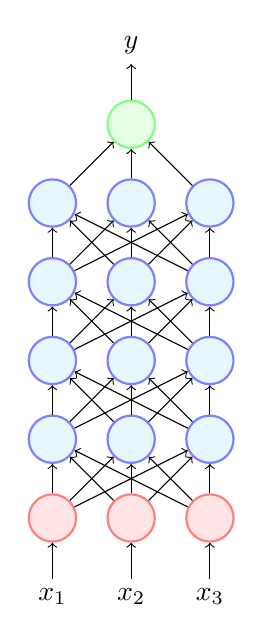
\begin{tikzpicture}
					
	\node [input_neuron] (neuron01) at (7,4.5){} ;
	\node [input_neuron] (neuron02) at (8,4.5){};
	\node [input_neuron] (neuron03) at (9,4.5){} ;
	\node (input0) at (7,3.5) {$x_{1}$};
	\node (input1) at (8,3.5) {$x_{2}$};
	\node (input2) at (9,3.5){$x_{3}$};
	
	\node [hidden_neuron] (neuron51) at (7,5.5){}  ;
	\node [hidden_neuron] (neuron52) at (8,5.5){}  ;
	\node [hidden_neuron] (neuron53) at (9,5.5){}  ;
	
	\node [hidden_neuron] (neuron11) at (7,6.5){}  ;
	\node [hidden_neuron] (neuron12) at (8,6.5){}  ;
	\node [hidden_neuron] (neuron13) at (9,6.5){}  ;
	\node [hidden_neuron] (neuron21) at (7,7.5){}  ;
	\node [hidden_neuron] (neuron22) at (8,7.5){}  ;
	\node [hidden_neuron] (neuron23) at (9,7.5){}  ;
	\node [hidden_neuron] (neuron31) at (7,8.5){}  ;
	\node [hidden_neuron] (neuron32) at (8,8.5){}  ;
	\node [hidden_neuron] (neuron33) at (9,8.5){}  ;
	%\node [output_neuron] (neuron41) at (7,9.5)  ;
	\node [output_neuron] (neuron42) at (8,9.5){}  ;
	%\node [output_neuron] (neuron43) at (9,9.5)  ;
	
	%\node (output0) at (7,10.5){$y_1$};
	\node (output1) at (8,10.5){$y$};
	%\node (output2) at (9,10.5){$y_3$};
	
	\draw[->](neuron01) -- (neuron51);
	\draw[->](neuron01) -- (neuron52);
	\draw[->](neuron01) -- (neuron53);
	\draw[->](neuron02) -- (neuron51);
	\draw[->](neuron02) -- (neuron52);
	\draw[->](neuron02) -- (neuron53);
	\draw[->](neuron03) -- (neuron51);
	\draw[->](neuron03) -- (neuron52);
	\draw[->](neuron03) -- (neuron53);
	
	\draw[->](neuron51) -- (neuron11);
	\draw[->](neuron51) -- (neuron12);
	\draw[->](neuron51) -- (neuron13);
	\draw[->](neuron52) -- (neuron11);
	\draw[->](neuron52) -- (neuron12);
	\draw[->](neuron52) -- (neuron13);
	\draw[->](neuron53) -- (neuron11);
	\draw[->](neuron53) -- (neuron12);
	\draw[->](neuron53) -- (neuron13);
	
	\draw [->] (neuron11) -- (neuron21);
	\draw [->] (neuron11) -- (neuron22);
	\draw [->] (neuron11) -- (neuron23);
	\draw [->] (neuron12) -- (neuron21);
	\draw [->] (neuron12) -- (neuron22);
	\draw [->] (neuron12) -- (neuron23);
	\draw [->] (neuron13) -- (neuron21);
	\draw [->] (neuron13) -- (neuron22);
	\draw [->] (neuron13) -- (neuron23);
	
	\draw [->] (neuron21) -- (neuron31);
	\draw [->] (neuron21) -- (neuron32);
	\draw [->] (neuron21) -- (neuron33);
	\draw [->] (neuron22) -- (neuron31);
	\draw [->] (neuron22) -- (neuron32);
	\draw [->] (neuron22) -- (neuron33);
	\draw [->] (neuron23) -- (neuron31);
	\draw [->] (neuron23) -- (neuron32);
	\draw [->] (neuron23) -- (neuron33);
	
	%\draw [->] (neuron31) -- (neuron41);
	\draw [->] (neuron31) -- (neuron42);
	%\draw [->] (neuron31) -- (neuron43);
	%\draw [->] (neuron32) -- (neuron41);
	\draw [->] (neuron32) -- (neuron42);
	%\draw [->] (neuron32) -- (neuron43);
	%\draw [->] (neuron33) -- (neuron41);
	\draw [->] (neuron33) -- (neuron42);
	%\draw [->] (neuron33) -- (neuron43);
	
	%\draw[->] (neuron41) -- (output0);
	\draw[->] (neuron42) -- (output1);
	%\draw[->] (neuron43) -- (output2);
	
	\draw[->] (input0) -- (neuron01);
	\draw[->] (input1) -- (neuron02);
	\draw[->] (input2) -- (neuron03);
	
\end{tikzpicture}
			\end{center}
						
		\end{overlayarea}
	\end{columns}
\end{frame}
\fi
%%%%%%%%%%%%%%%%%%%%%%%%%%%%%%%%%%%%%%%%%%%%%%%%%%%%%%%%%%%%%%%%%%%%%%%%%%%%%%%%%%%%%%%%%

\begin{frame}
	\begin{center}
		So what has happened since 2006-2009?
		
	\end{center}
	    
\end{frame}

%%%%%%%%%%%%%%%%%%%%%%%%%%%%%%%%%%%%%%%%%%%%%%%%%%%%%%%%%%%%%%%%%%%%%%%%%%%%%%%%%%%%%%%%%

\begin{frame}
	\begin{block}{Deep Learning has evolved}
		\begin{itemize}[<+->]
			\justifying
			\item \textcolor{gray}{Better optimization algorithms}
			\item \textcolor{gray}{Better regularization methods}
			\item Better activation functions
			\item Better weight initialization strategies
		\end{itemize}
		
	\end{block}
\end{frame}